\definecolor{gray}{gray}{0.6}
\section{Quality Requirements}

This section describes the quality requirements for the game and will briefly describe all requirements under each quality requirement. Each requirement will be described with a quality attribute scenario that looks like this \cite{qualityAttribute}:

\begin{itemize}
	\item {\bf Source of stimulus:} Human, computer, or other actor that generates the stimulus
	\item {\bf Stimulus:} Condition that needs to be considered when it arrives at a system
	\item {\bf Environment:} The stimulus occurs within certain conditions
	\item {\bf Artifact:} Some artifact is stimulated 
	\item {\bf Response:} The activity undertaken after the arrival of the stimulus
	\item {\bf Response measure:} When the response occur, it should be measured in some fashion so that the requirement can be tested.
\end{itemize}

\begin{figure}[!hr]
	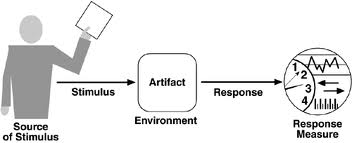
\includegraphics{pictures/qualityAttribute.jpg}
	\caption{Quality attribute scenario}
\end{figure}

{\bf Priority of quality attributes:} It is not possible to meet all quality requirements because some decisions will affect others. This will result in a priority of the quality attributes that we need to meet and some that are less important. We have picked two main quality attributes: Modifiability and performance.

\begin{itemize}
	\item {\bf Primary quality attribute: } Modifiability
	\item {\bf Secondary quality attributes: } Performance
\end{itemize}


\subsection{Modifiability}

Modifiability \cite{attributes} is about the cost of change. It brings up two concerns: 
What can change (the artifact)? 
When is the change made and who makes it (the environment)? 
Once a change has been specified, the new implementation must be designed, 
implemented, tested, and deployed. All of these actions take time and money, both of which can be measured.

Helgelandskraft (the customer) wanted the possibility for further development on the game. The developers
have to keep in mind that the game is developed in a such way that the customer can continue
the development after the delivery. If the game is made in a way that changes are hard to implement, 
the customer would need to use a lot of resources in sense of time and money, and that is the main 
reason for this to be the primary quality attribute.

Changes the customer might want to add to the game is more buildings and more obstacles to take
the game to a more complex state. Good models have therefore been added so that it will be easy for 
the customer to make further development on this part.

\subsection*{M1: Add new elements}
In the game a small set of elements like powerplants, houses, powerlines, etc. has been specified.
In order to have the oppertunity to add new buildings a model for each element with specific attributes has been made. When a developer wants to add more elements, he or she can use these models and easily add the wanted parameters. 

\begin{table}[H]
\begin{tabular}{| l | l |}
	\hline
	\rowcolor{gray}
	{\bf Portion of scenario} & {\bf Values} \\ \hline
	Source of stimulus & Developer\\ \hline
	Stimulus & Add new elements to the game\\ \hline
	Environment & Design time \\ \hline
	Artifact & Code \\ \hline
	Response & Modification is made with no side effects\\ \hline
	Response Measure & 1 hour\\ \hline
\end{tabular}
\caption{Modifiability scenario}
\end{table}

\subsection* {M2: Increase game difficulty}
If the game is made to easy for the user it is possible for the developer to adjust the
parameters in the models. The difficulty of the game is based on these parameters.

\begin{table}[H]
\begin{tabular}{| l | l |}
	\hline
	\rowcolor{gray}
	{\bf Portion of scenario} & {\bf Values} \\ \hline
	Source of stimulus & Developer\\ \hline
	Stimulus & Modify the difficulty in the game\\ \hline
	Environment & Design time \\ \hline
	Artifact & Code \\ \hline
	Response & Modification is made with no side effects\\ \hline
	Response Measure & 1 hour\\ \hline
\end{tabular}
\caption{Performance scenario}
\end{table}

\subsection{Performance}

Performance\cite{attributes} is about timing. Different events occur and the system must respond to them. Performance is concerned about how long it takes to respond to events. Performance becomes complicated because of the number of event sources and arrival pattern.

Performance is very important for games. If the game takes too long responding to user input, the game feels slugish and the player is likely to quit playing. The game also has it's own logic running in parallel to the user interacting with the game which affects the users perception of the game. If the game runs at a slow pace the user experience suffers as a result.

\subsection*{P1: Rendering (Repaint)}
When changes occure to the game models, the screen should identify if the change 
is visible on the screen. If the change can be seen, the screen should repaint 
that part of the display at the beginning of the next game update.

\begin{tabular}{| l | l |}
	\hline
	\rowcolor{gray}
	{\bf Portion of scenario} & {\bf Values} \\ \hline
	Source of stimulus & Game models\\ \hline
	Stimulus & Change to the internal state of game model\\ \hline
	Environment & Game run time \\ \hline
	Artifact &  Game \\ \hline
	Response & Identify visibility of state change\\ \hline
	Response Measure & Less than 16 ms\\ \hline
\end{tabular}

\subsection{Other Quality Attributes}
\subsection*{Usability: } The group do not have the main focus on this quality attribute, but because this is a game that is supposed to be played by a variety of people, it has to be considered to make the game easy to use. Instructions in the main menu has been added to help the user get started.\cite{attributes}

\subsection*{Testability: } Since the game is made as a prototype, the focus has been on having
test on the main functionality so the customer can run test under further development.
In order to have test, testable code needs to be written.\cite{attributes}

\subsection*{Compitability: } The game has to run on different kinds of platforms. A cross-platform framework has been chosen for development to make it it easier to adapt to new platforms.
